%   Filename    : chapter_1.tex 
\chapter{Introduction}
\label{sec:researchdesc}    %labels help you reference sections of your document
 

Mental health problems have been prevalent among young adults \cite{hunt:2010:mental}. But, due to COVID-19 and the infamous remote learning setup, a major increase in the population of students who are in their postgraduate education experiences depression and anxiety has increased \cite{qiu2020nationwide}. Mental health awareness is being strengthened in schools \cite{hoven2008worldwide}. However, some research has suggested that there are help-seeking barriers – negative attitudes toward seeking help, limited access to treatment, confidentiality, and self-reliance – that prevent students from seeking help \cite{rickwood2005young}. The study aimed to understand the need for a proper online modality to access counseling services for better mental health awareness. The study examined prevalent mental health problems among students and the advantages of online counseling to both students and counselors in schools. 

\section{Overview of the Current State of Technology}
\label{sec:overview}

The COVID-19 situation in the Philippines still prohibits face-to-face classes, therefore, causing a lot of implications on students’ mental health. Throughout these times, students from the University of the Philippines-Miagao (UPV-M) have been more prone to mental health problems such as depression and anxiety. The University has its own intervention program for mental health - The Guidance and Counseling Services (UPV-GCS) Unit is available online through social media platforms in catering to students during remote learning setup. 

The use of social media platforms offers convenience and ease of access. However, providing mental health services in any of the platforms like Facebook, Twitter, and Instagram hinders the quality of services because of threats such as user profiling and unstable server issues.  Also, school e-mail is used to promote mental health services. The scope is the wide range of students who have access to their school e-mail accounts. But nowadays, e-mail is ignored due to messaging applications, thus, results in low participation of students. 

On the Guidance and Counseling Services (UPV-GCS) Facebook page, a student can view posts regarding available services as well as programs from other institutions that offer other counseling services and, a student can inquire and book an appointment through Facebook messenger. To book an appointment, (1) The student shall visit the Facebook page and click on the “Book Now” button on its homepage, (2) A Request Date and Time window will popup displaying the available dates and corresponding time which the student can choose from, (3) Automatically, an Additional Information window will be asked for the student’s phone number and appointment notes which are optional only, and (4) The student can click on “Request Appointment” button which will then generate an approval form of some sort into the Messenger chat panel between the Facebook page and the student. If approved, the student is given the choices for modalities to be used. This information is passed to the counselor who will accommodate the appointment of the student, and the online counseling will be taken care of by the counselor in their personal account. 
   
%\textcolor{red}{This section ends with a discussion on the problem/s faced by or that still exist in the specific
%technology or field (e.g., limitations of existing software or algorithms). 
%The problem statement would lead to the research objectives.}


%It is   easy to include a figure in JPG or PNG format as shown in the  following example.  
%Make sure that you explain what the figure is all about, and that you refer to your figure.  
%For example, \figref{fig:disneystock} shows a graph of the performance of Disney stock from the 1980s to 2012.
  
%--- the following example shows how to include a figure in PNG format
%\begin{figure}[t]                %-- use [t] to place figure at top, [b] to place at the bottom, [h] for here
 %  \centering                    %-- use this to center the figure
 %  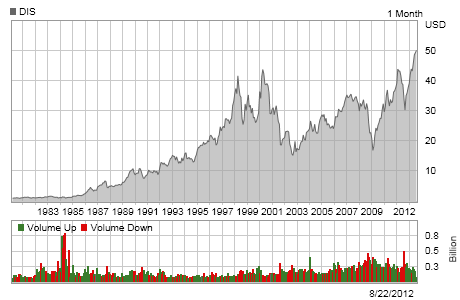
\includegraphics{DisneyChart.png}      %-- include image file named as "disneychart.png" 
 %  \caption{This is the figure's caption -- Disney stock chart.
 %  	Captions should fully describe the figure in a concise manner  such that there is not need to refer to the text when figuring out the graphic.}
 %   \label{fig:disneystock}
%\end{figure}


%Some notes on citing references.   
%When using APA format, the author-date method of citation is  followed.   
%This means that the author's last name and the year of publication for the source should  appear in the text, and a complete reference should appear in the reference list.

% Examples:
%     	Smith (1970) compared reaction times . . .
%     	In a recent study of reaction times (Smith, 1970), . . .   
%     	In 1970, Smith compared reaction times . . .
%	    Smith, et al., (1970) compared reaction times . . .
%     	In a recent study of reaction times (Smith, et al., 1970), . .
%     	In 1970, Smith, et al., compared reaction times . . .

%Here are some examples on how to do the referencing (note author's name and years are different from commented examples).  
%For APA citation details, refer to \url{http://www.ctan.org/tex-archive/biblio/bibtex/contrib/apacite/}. 

%\begin{itemize}
% \item \citeA{kartch:2000:ERA} compared reaction times...
% \item In a recent study of reaction times \cite{kartch:2000:ERA}...
% \item In \citeyearNP{kartch:2000:ERA}, \citeauthor{kartch:2000:ERA} compared reaction times...
% \item \shortciteA{fedkiw:2001:VSO} compared reaction times... 
% \item In a recent study of reaction times \cite{fedkiw:2001:VSO}...
% \item In \citeyearNP{fedkiw:2001:VSO}, \shortciteauthor{fedkiw:2001:VSO}, compared reaction times...
%\end{itemize}

%The following are references from journal articles \cite{Park:2006:DSI, Pellacini:2005:LAH, sako:2001:SSB}.
% Here's an MS thesis document \cite{yee:2000:SSA}, and this is from PhD dissertation \cite{kartch:2000:ERA}. 
% For a book, reference is given as  \cite{parke:1996:CFA}. 
% Proceedings from a conference samples are \cite{Jobs95, fedkiw:2001:VSO, levoy:2000:TDM}.  
% The sample bibliography file named \textbf{myreferences.bib} is from the SIGGRAPH \LaTeX{}  template.  
% You can use a text editor to view the contents of the bib file.  
%% It is your task to create your own bibliography file.  
% For those who downloaded papers from ACM or IEEE sites, there is a BibTeX link that you can click; thereafter, you just simply need to copy and paste the BibTeX entry into your %own bibliography file.

%The following shows how to include a program source code (or algorithm).  
%The verbatim environment, as the name suggests, outputs text (including white spaces) as is...
%
%\begin{verbatim}
%               #include <stdio.h>
%               main()
%               {
%                    printf("Hello world!\n");
%               }
%\end{verbatim}

\section{Problem Statement}
%\textcolor{red}{DO NOT FORGET to write the statement of the research problem here, i.e., before the Research Objectives.}
\begin{itemize}
\item Mental health awareness
	\begin{itemize}
	\item During these trying times, UPV students tend to experience anxiety, stress, time pressure, mental exhaustion, and negativity which can be too much to handle and cause a greater mental health problem. Thus, UPV students should be able to check on their mental health by talking with experienced mental health providers. 
	\end{itemize}
\item No site for counseling
	\begin{itemize}
	\item One of the UP benefits is having free consultation from the Guidance Office. However, due to the remote learning setup, this benefit is hard to avail since there is no official site where students can go and schedule an appointment, or a 	guidance counselor to post counseling offers to students.
	\end{itemize}
\end{itemize}


\section{Research Objectives}
\label{sec:researchobjectives}

\subsection{General Objective}
\label{sec:generalobjective}
The objectives of the study is to design a secure online platform where the UPV-GCS guidance counselors and students connect with each other and to avail counseling services that may help students to have an accessible mental health service platform. 
 
%\item To understand the need for a proper online modality for the UPV-M students to access and avail counseling services.  
%\item To show how important it is to have an accessible mental health service platform for the UPV community.  
%\item To design a secure online platform where the UPV-GCS guidance counselors and students connect with each other.  
%\end{enumerate}
  
\subsection{Specific Objectives}
\label{sec:specificobjectives}

%
%  \begin{comment} ... \end{comment} is used for multiple lines of comment
%
During this study, a system-website is to be created according to the needs of a guidance counselor to make their services available online, and to the needs of students to avail counseling services in an easy way. 
\\*
\newline \textbf{UPV Guidance Counseling System}
\newline
\newline This system-website may include features such as: 
\begin{itemize}
\item Messaging on this site
	\begin{itemize}
	\item This feature is direct messaging within the site between students and guidance counselors. 
	\end{itemize}
\item Select services
	\begin{itemize}
	\item This feature is a great help to showcase the services available for UPV students. 
		\begin{itemize}
		\item Counseling Services 
		\item  Psychological Assessment and Evaluation 
		\item Referral Service 
		\item Peer Psychosocial Support: The Buddy System  
		\end{itemize}
	\end{itemize}
\item Schedule an appointment 
	\begin{itemize}
	\item The feature on the website will ask for the preferred schedule for an appointment while displaying the availability hours of the guidance counselor.
	\end{itemize}
\end{itemize}



\begin{comment}
This subsection is an elaboration of the general objective.  
It states the specific steps that must be undertaken to accomplish the general objective.  
These objectives must be \textbf{S}pecific, \textbf{M}easurable, \textbf{A}ttainable, \textbf{R}ealistic, \textbf{T}ime-bounded.  
A specific objective start with ``to $<$verb$>$'' for example: to design/survey/review/analyze.

Studying a particular programming language or development tool (e.g., to study Windows/Object-Oriented/Graphics/C++ programming) to  accomplish the general objective is inherent in all thesis and, therefore, must not be included here.
\end{comment}


\begin{comment}
% IPR acknowledgement: the following sentences and examples are from Ethel Ong's slides 
%     on Research Objectives
How to formulate your research objectives:
1. Identify what research steps do you need to perform to achieve your general objective.
2. Identify the questions that must be answered for you to achieve your general objective.
    Thereafter, convert these questions into action statements

Example #1:

Research Question:
  What are the general features of a web-based learning environment?

Specific Objective:
   To review existing web-based learning environment that teaches language learning for children


Example #2:

Research Question:
   How will you represent commonsense knowledge for use by computer systems?

Specific Objective:
   To identify knowledge representation approaches used by existing story generation systems

Example #3:
Research Question:
   What types of storytelling knowledge are needed to generate stories?

Specific Objective:
    To identify the different types of storytelling knowledge used in generating stories

Example #4:
Research Question:
    What machine learning approaches will you utilize?

Specific Objective:
    To determine existing machine learning algorithms [that can be used in training the computer system to detect cyberbullying cases] 

Example #5: Research Question:
    How will your research output be evaluated?

Specific Objective:
    To define evaluation metrics for validating the accuracy of the translation

\end{comment}

%
%  The following are example specific objectives; replace them with your own 
%

\begin{comment}
   \item To review related literature, compare and contrast existing algorithms (on what problem?);
   \item To develop a new algorithm (for what purpose?)
   \item To analyze the algorithm (based on what criteria?)
\end{comment}


\section{Scope and Limitations of the Research}
\label{sec:scopelimitations}

The study is limited only to the University of the Philippines Visayas-Miagao (UPV-M) students who are officially enrolled and to the UPV-GCS guidance counselors who are officially hired. The website will accommodate students who seek help for their mental health in these trying times by being able to inquire about services and book an appointment to avail themselves of a service. The system will be for online guidance and counsel, and record-keeping such that UPV-GCS will be able to accept counseling appointments scheduled by the students and generate a report according to important demographic details. 

\begin{comment}

%
% IPR acknowledgement: the sentences inside this comment are from Ethel Ong's slides on Scope and Limitations of the Research
%
Generally, one paragraph should be allotted for each of your research objectives.

Each paragraph contains a brief overview of the concept/theory and the purpose of doing the associated objective.

Each paragraph also includes a description of the scope/limitation of your study.

* Please refer to the slides for examples.

\end{comment}


\section{Significance of the Research}
\label{sec:significance}

The completion of this study will help the researchers to build a formal system-website where counselors can post their service offerings, store and access confidential data about their clients, and keep reports for analysis purposes, and students can ask and book an appointment of the desired service, as well as direct message their preferred counselor. 

This would be a significant help to campaign mental health awareness. Students will have a venue where they can access mental health services without external help-seeking barriers. Guidance counselors will be able to distinguish essential mental health needs of students and improve their services accordingly. Thus, this research is not only to promote mental health awareness but also to improve the status of mental health in the university. 



\begin{comment}
This section explains why research must be done in this area.
 It rationalizes the objective of the research with that of the stated problem. 
 Avoid including sentences such as ``This research will be beneficial to the proponent/department/college'' as this is already an inherent requirement of all BSCS majors.  Focus on the research's contribution to the Computer Science field.

The following are guide questions that may help your formulate the significance of your research. 


%
% IPR acknowledgement: the following list of items are from Ethel Ong's slides on Significance of the Research
%
\begin{itemize}
\item  What is the relevance of your work to the computer science community? 

\begin{itemize} 
\item What will be your technical contributions, in terms of algorithms, or approaches, or new domain? 
\item What is your value-added compared to existing systems? 
\end{itemize}

\item What will be your contributions to society in general? 
    \begin{itemize}
      \item Who will benefit from your system? 
      \item Who are your target users and how will this system benefit them? 
   \end{itemize}
\end{itemize}


If applicable, describe possible commercialization and/or innovation in your research.
\end{comment}


